
% Geophysical equations (converted from handwritten notes)
% Source: user-provided PDF notes
\documentclass[11pt,a4paper]{article}
% Custom notes package provided by the user
\usepackage{notes}

% TikZ helpers for diagrams
\usetikzlibrary{arrows.meta,calc}
\usetikzlibrary{
    decorations.pathmorphing,
    decorations.pathreplacing,
    decorations.markings,
    arrows.meta
}
% --- Equation numbering ---
% Continuous equation numbering is the LaTeX default (no per-section reset).
% We intentionally do NOT call \numberwithin{equation}{section}.

\title{Geophysical Equations and Field Operators}
\author{Derrick Hasterok}
\date{\today}

\begin{document}
\maketitle

\section{What is Geophysics?}
Geophysics is the study of the physical properties of the Earth (and other planetary bodies) and the physical processes that operate on or within them, using observations, modeling, and controlled experiments on physical fields (??). A \emph{field} is any quantity that can be specified throughout space (and possibly time), with a position and a value (magnitude and, for vectors, direction).

\paragraph{Examples of fields}
\begin{itemize}
  \item Scalar fields: temperature \(T(\vb{x})\), elevation \(z(\vb{x})\), composition variables (e.g., modal fraction) (??).
  \item Vector fields: gravitational acceleration \(\vb{g}(\vb{x})\), wind velocity \(\vb{u}(\vb{x})\), magnetic field \(\vb{B}(\vb{x})\).
  \item Tensor fields: Cauchy stress \(\bm{\sigma}(\vb{x})\), strain \(\bm{\varepsilon}(\vb{x})\).
\end{itemize}

A field can be represented as a function $f(\vb{x})$ mapping each position $\vb{x} = (x,y,z)$ to a value in $\mathbb{R}$, $\mathbb{R}^3$, or a tensor space depending on type.

\section{Describing Change: Derivatives and the Gradient}
For a scalar field $f(\vb{x})$, the rate of change along coordinate directions is given by partial derivatives:
\begin{equation}
  \pdv{f}{x},\; \pdv{f}{y},\; \pdv{f}{z} .
\end{equation}
The \emph{gradient} of $f$ is the vector field
\begin{equation}
  \grad f = \left( \pdv{f}{x},\; \pdv{f}{y},\; \pdv{f}{z} \right) .
\end{equation}

\begin{figure}[h]
  \centering
  \begin{tikzpicture}[scale=1]
    % axes
    \draw[-{Latex}] (-0.2,0) -- (4.2,0) node[below]{$x$};
    \draw[-{Latex}] (0,-0.2) -- (0,3) node[left]{$f$};
    % curve and tangent
    \draw[thick,BrickRed] plot[smooth] coordinates{(0.2,0.4) (0.8,0.8) (1.6,1.3) (2.4,1.9) (3.2,2.4) (3.8,2.6)};
    \fill (2.4,1.9) circle (1.2pt) node[above right]{$(x,f)$};
    \draw[OliveGreen,thick] (1.8,1.5) -- (3.0,2.3);
    \node[OliveGreen!70!black] at (3.2,2.3) {$\displaystyle \pdv{f}{x}$};
  \end{tikzpicture}
  \caption{Slope of a scalar field along $x$ at a point (schematic).}
\end{figure}

\section{Divergence: Measuring Outflow of a Vector Field}
For a vector field $\vb{F} = (F_x,F_y,F_z)$, the \emph{divergence} is
\begin{equation}
  \div{\vb{F}} = \pdv{F_x}{x} + \pdv{F_y}{y} + \pdv{F_z}{z} .
\end{equation}
Physically, $\nabla\cdot\vb{F}$ measures the net ``density change'' or source strength at a point. A classic example is a radially expanding flow (e.g., an explosion), which has positive divergence away from the source.

\begin{figure}[h]
  \centering
  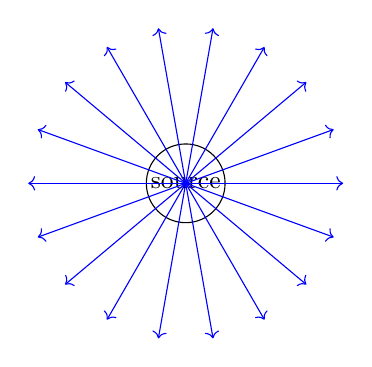
\begin{tikzpicture}[scale=1]
    \draw (0,0) circle (0.5) node{\small source};
    \foreach \ang in {0,20,...,340} {
      \draw[->,Blue] (0,0) -- ({2*cos(\ang)},{2*sin(\ang)});
    }
  \end{tikzpicture}
  \caption{Schematic of a diverging vector field (explosive‐like outflow).}
\end{figure}

\section{Divergence Theorem and the Laplacian}
Over a volume $V$ with boundary surface $\partial V$ and outward unit normal $\vu{n}$, the divergence theorem states
\begin{equation}
  \iiint\limits_V (\div{\vb{F}})\,\dd{V} = \iint\limits_{\partial V} \vb{F} \cdot \vu{n}\,\dd{S} .
\end{equation}

The \emph{Laplacian} of a scalar field is the divergence of its gradient:
\begin{equation}
  \laplacian f \equiv \div (\nabla f) = \pdv[2]{f}{x} + \pdv[2]{f}{y} + \pdv[2]{f}{z} .
\end{equation}
It measures curvature of the field and appears ubiquitously in geophysical governing equations.

\begin{figure}[h]
  \centering
  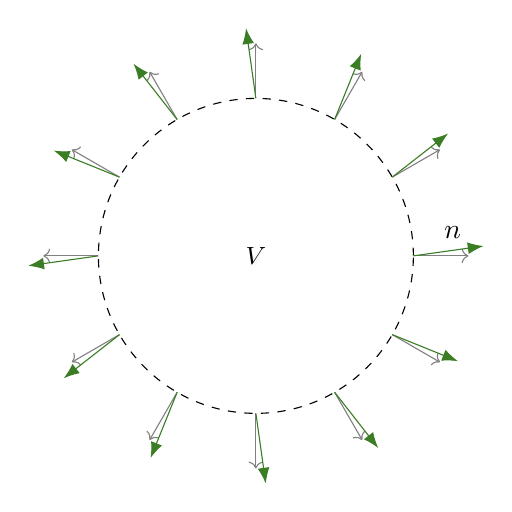
\begin{tikzpicture}[scale=1]
    % Draw a Gaussian surface around a point
    \draw[dashed] (0,0) circle (2);
    \node at (0,0) {\small $V$};
    % outward normals and F
    \foreach \ang in {0,30,...,330} {
      \draw[->,Gray] ({2*cos(\ang)},{2*sin(\ang)}) -- ++({0.7*cos(\ang)},{0.7*sin(\ang)});
      \draw[-{Latex[length=2mm]},OliveGreen] ({2*cos(\ang)},{2*sin(\ang)}) -- ++({0.9*cos(\ang+8)},{0.9*sin(\ang+8)});
    }
    \node at (2.5,0.3) {$\vu{n}$};
  \end{tikzpicture}
  \caption{Flux through a closed surface $\partial V$ equals volume integral of $\div {\vb{F}}$ (schematic).}
\end{figure}

\section{Canonical Field Equations}
\subsection{Poisson and Laplace Equations}
Many static (time‐independent) geophysical fields satisfy Poisson's equation
\begin{equation}
  \laplacian \Phi(\vb{x}) = S(\vb{x}) ,
\end{equation}
where $\Phi$ is a potential and $S$ is a source term determined by the underlying physics. In source‐free regions ($S=0$), this reduces to Laplace's equation
\begin{equation}
  \laplacian \Phi = 0 .
\end{equation}

\subsection{Examples}
\begin{itemize}
  \item Gravitation (Newtonian, scalar potential $\Phi_g$): \; $\laplacian \Phi_g = 4\pi G\,\rho$.  \; (units ``fudge factor'' comment in notes: ??)
  \item Steady heat conduction (temperature $T$ with volumetric heat production $A$ and conductivity $k$): \; $\laplacian T = -\dfrac{A}{k}$ (sign/convention in notes: ??).
  \item Magnetostatics (scalar magnetic potential under curl‐free conditions): \; form depends on magnetization $\vb{M}$ and permeability $\mu$ (exact form in notes: ??).
\end{itemize}

\section{Diffusion}
Time‐dependent smoothing (diffusive) processes satisfy
\begin{equation}
  \pdv{u}{t} = \kappa\,\laplacian u + S(\vb{x},t) ,
\end{equation}
with diffusivity $\kappa$ (``diffusion constant'' in notes). In geothermics, $u\equiv T$ and $\kappa$ is the thermal diffusivity (the notes suggest we may not use this often here: ??).

\section{Constitutive Relations (Statics)}
\begin{itemize}
  \item Electrical conduction (Ohm's law): $\vb{J} = \sigma\,\vb{E}$.
  \item Magnetics: $\vb{B} = \mu\,\vb{H}$; with magnetization, $\vb{B} = \mu_0(\vb{H}+\vb{M})$ (specific form referenced in notes: ??).
\end{itemize}

\section{Wave Phenomena}
Propagating fields typically satisfy a second‐order wave equation
\begin{equation}
  \pdv[2]{u}{t} = v^2\,\nabla^2 u ,
\end{equation}
where $v$ is the propagation speed.

\paragraph{Seismology.} In elastic media, compressional (P) and shear (S) waves have speeds $v_p$ and $v_s$ respectively (details and exact parameter relations deferred in the notes: ??).

\section{Electromagnetics (constants and vacuum relations)}
The speed of light in vacuum is related to the permittivity and permeability of free space by
\begin{equation}
  c = \frac{1}{\sqrt{\mu_0\,\epsilon_0}} .
\end{equation}
Further wave equations for $\vb{E}$ and $\vb{H}$ in free space (if needed in these notes: ??).

\section{Fundamental Quantities}
\begin{description}
  \item [Mass] $m$: amount of matter (units: kg).
  \item [Position] $\vb{x}=(x,y,z)$ with unit vectors $\vu{i},\vu{j},\vu{k}$ (units: \si{m}). Magnitude $r=\norm{\vb{x}}$.
  \item [Velocity] $\vb{v}=\dd{\vb{x}}{t}$ (units: \si{m.s^{-1}}).
  \item [Acceleration] $\vb{a}=\dd{\vb{v}}{t}=\d[2]{\vb{x}}{t}$ (units: \si{m.s^{-2}}).
  \item [Force] $\vb{F}$: interaction that changes motion. Newton's 2nd law: $\vb{F}=m\,\vb{a}$ (units: \si{N} = \si{kg.m.s^{-2}}).
\end{description}

\paragraph{Static equilibrium.} At rest does not imply ``no forces''; rather, forces balance (e.g., gravity vs.~normal reaction at the ground), so net force is zero: $\sum\vb{F}=\vb{0}$.

\section{Work and Energy}
Work by a force along a path $\mathcal{C}$: \; $W=\displaystyle\int_{\mathcal{C}} \vb{F}\cdot\dd{\vb{s}}$ (units: J = \si{N.m}). The dot product projects the force along the direction of motion. Kinetic energy $K=\tfrac12 m\,v^2$.

\paragraph{Work--energy relation.} Using $\dd{K}{t}=\vb{F}\cdot\vb{v}$, integration along the path gives the change in kinetic energy equals work done.

\section{Potential and Path Independence}
When the work between two points depends only on endpoints (not the path), the field is conservative and admits a potential $\Phi$ with $\vb{F} = -\nabla\Phi$ (sign conventions in the notes mention ``force is gradient of work''; adopt $\vb{F} = -\nabla\Phi$ here and reconcile with class convention: ??).

\begin{align}
  W_{P\to Q} &= \int_{\mathcal{C}} \vb{F}\cdot\dd{\vb{s}} = -\big[\Phi(Q)-\Phi(P)\big].
\end{align}

Differential form: $\nabla\times\vb{F}=\vb{0}$. Integral form: line integral is path independent.

\section{Field Types and Representations}
\begin{itemize}
  \item \textbf{Scalar field} $T(\vb{x})$ (e.g., temperature, elevation).
  \item \textbf{Vector field} $\vb{g}(\vb{x}),\,\vb{B}(\vb{x})$.
  \item \textbf{Tensor field} $\mat{\sigma}(\vb{x}),\,\mat{\varepsilon}(\vb{x})$.
\end{itemize}

\subsection{Visualizations}
\paragraph{Quiver plot (vectors).}
\begin{figure}[h]
  \centering
  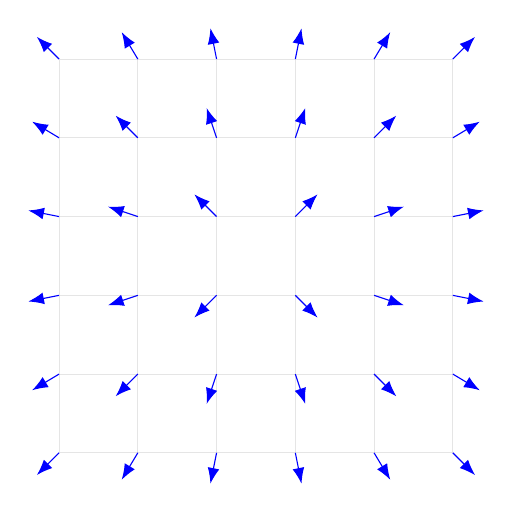
\begin{tikzpicture}[scale=1]

    % grid
    \foreach \x in {0,...,5} {
        \draw[gray!20] (\x,0) -- (\x,5);
    }
    \foreach \y in {0,...,5} {
        \draw[gray!20] (0,\y) -- (5,\y);
    }

    % simple radial field arrows
    \foreach \x in {0,...,5} {
        \foreach \y in {0,...,5} {

            \pgfmathsetmacro{\dx}{\x-2.5}
            \pgfmathsetmacro{\dy}{\y-2.5}
            \pgfmathsetmacro{\r}{sqrt(\dx*\dx+\dy*\dy)+1e-6}

            \draw[-{Latex[length=2mm]},blue]
            (\x,\y) -- ++({0.4*\dx/\r},{0.4*\dy/\r});

        }
    }

  \end{tikzpicture}
  \caption{Quiver depiction of a simple radial vector field.}
\end{figure}

\paragraph{Field lines.}
\begin{figure}[h]
  \centering
  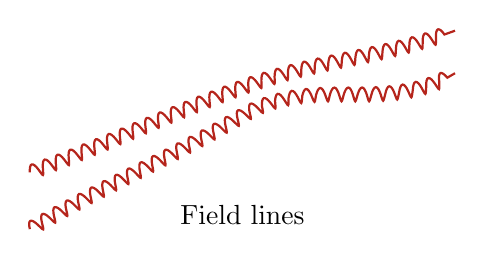
\begin{tikzpicture}[scale=0.9]
    % streamline-like curves
    \draw[BrickRed,thick,decorate,decoration={coil,aspect=0.15,segment length=5pt}] (-3,-1) to[out=20,in=200] (0,0.2) to[out=20,in=200] (3,1.0);
    \draw[BrickRed,thick,decorate,decoration={coil,aspect=0.15,segment length=5pt}] (-3,-1.8) to[out=30,in=210] (0,-0.2) to[out=30,in=210] (3,0.4);
    \node at (0,-1.6) {Field lines};
  \end{tikzpicture}
  \caption{Sketch of field/force lines.}
\end{figure}

\begin{figure}[h]
  \centering
  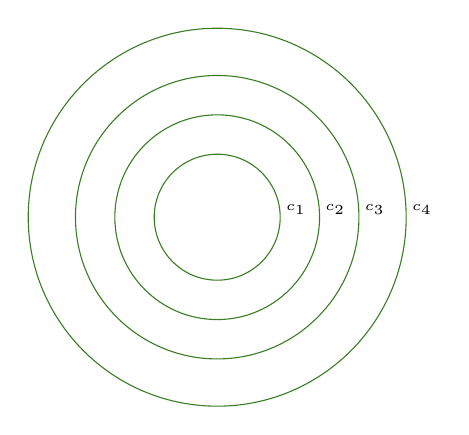
\begin{tikzpicture}[scale=1]

    % concentric contours
    \foreach \r [count=\k] in {0.8,1.3,1.8,2.4} {
      \draw[OliveGreen] (0,0) circle (\r);
      \node at (\r+0.2,0.1) {\tiny $c_{\k}$};
    }

  \end{tikzpicture}
  \caption{Iso-contours (perpendicular to field lines in conservative fields).}
\end{figure}

\section{Continuity and Differentiability}
A function is continuous if it can be traced without breaks. Differentiability additionally requires the slope to be well-behaved (left and right derivatives agree). Points with corners or cusps are non-differentiable.

\section{Superposition}
In linear systems, fields add. For sources $S_1, S_2$, the resulting field is $f=f_1+f_2$ (additivity) and scales with source strength (homogeneity). This principle underlies many constructions in potential theory.

\begin{align}
  f(\alpha S) &= \alpha f(S),\\
  f(S_1+S_2) &= f(S_1)+f(S_2).
\end{align}

\begin{figure}[h]
  \centering
  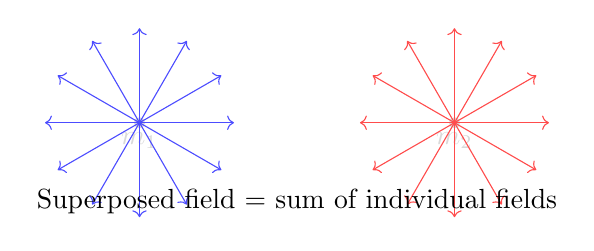
\begin{tikzpicture}[scale=1]
    \fill[gray!30] (-2,0) circle (0.07) node[below]{$m_1$};
    \fill[gray!30] ( 2,0) circle (0.07) node[below]{$m_2$};
    \foreach \ang in {0,30,...,330} {
      \draw[->,Blue!70] (-2,0) -- ++({1.2*cos(\ang)},{1.2*sin(\ang)});
      \draw[->,Red!70] ( 2,0) -- ++({1.2*cos(\ang)},{1.2*sin(\ang)});
    }
    \node at (0,-1.0) {Superposed field = sum of individual fields};
  \end{tikzpicture}
  \caption{Illustration of superposition from two sources.}
\end{figure}

\bigskip
\noindent\textit{Transcription notes:} Where the original handwriting or OCR was ambiguous, a ``??'' marker should be inserted during detailed equation derivations (none were strictly required in this summary; add if needed upon your review). Diagrammatic sketches have been redrawn schematically in TikZ.

% --- Optional bibliography placeholder (insert existing refs if any) ---
% \begin{thebibliography}{9}
% \bibitem{...} ...
% \end{thebibliography}

\end{document}
